\documentclass[unknownkeysallowed,14pt]{beamer}

\mode<presentation>
\usetheme{NCSUstat}
%% \setbeamercovered{transparent}
\usepackage[english]{babel}
\usepackage[latin1]{inputenc}
\usepackage{times}
\usepackage[T1]{fontenc}
\usepackage{booktabs}
\usepackage[absolute,overlay]{textpos}
\usepackage{tikz-cd}

% !TeX root = main.tex

\newtheorem{theorem}{Theorem}
\newtheorem{lemma}{Lemma}
\newtheorem{corollary}{Corollary}
\newtheorem{definition}{Definition}

\newcommand{\R}{\mathbb{R}}
\newcommand{\N}{\mathcal{N}}
\renewcommand{\O}{\mathcal{O}}
\newcommand{\e}{\varepsilon}
\newcommand{\Pers}{\mathcal{P}}
\newcommand{\dist}{\mathbf{d}}
\newcommand{\dmax}{\dist_{\mathrm{max}}}
\newcommand{\Cech}{\v Cech\xspace}
\newcommand{\cech}{\check{\mathcal{C}}}
\newcommand{\rips}{\mathcal{R}}
\newcommand{\T}{\mathcal{T}}
\newcommand{\ball}{\mathbf{ball}}
\newcommand{\PPers}{\mathbb{P}}
\newcommand{\hf}{\hat{f}}
\renewcommand{\ker}{\mathbf{ker}\xspace}
\newcommand{\im}{\mathbf{im}\xspace}
\newcommand{\cok}{\mathbf{cok}\xspace}
\newcommand{\coim}{\mathbf{coim}\xspace}
\newcommand{\id}{\mathbf{1}}


\renewcommand{\restriction}{\mathord{\mid}}
\newcommand{\rest}{\mathord{\mid}}

\mathchardef\mhyphen="2D
\newcommand{\Z}{\mathbb{Z}}
\newcommand{\rad}{\mathrm{rad}}
\newcommand{\birth}{\mathrm{birth}}
\newcommand{\death}{\mathrm{death}}
\newcommand{\pers}{\mathrm{Pers}}
\newcommand{\bary}{\mathrm{Bary}}
\newcommand{\kbary}{k\mhyphen\mathrm{Bary}}
\newcommand{\kcover}{k\mhyphen\mathrm{Cover}}
\newcommand{\cent}{\mathrm{center}}
\newcommand{\JL}{\textsc{JL}\xspace}
\newcommand{\conv}{\mathrm{conv}}
\newcommand{\power}{\mathcal{P}}
\newcommand{\C}{\mathcal{C}}
\newcommand{\nrv}{\text{Nerve}}
\newcommand{\Hom}{\mathrm{Hom}}
\newcommand{\knrv}{k\mhyphen\mathrm{Nerve}}
\newcommand{\clique}{\mathrm{Clq}}
\newcommand{\F}{\mathcal{F}}
\newcommand{\G}{\mathcal{G}}
\newcommand{\Rips}{\mathrm{Rips}}
\newcommand{\projectionOf}[1]{\overline{#1}}
\newcommand{\Pbar}{\projectionOf{P}}
\newcommand{\Sbar}{\projectionOf{S}}
\newcommand{\Tbar}{\projectionOf{T}}
\DeclareMathOperator*{\argmin}{argmin}
\newcommand{\wfs}{\mathrm{wfs}}
\newcommand{\reach}{\mathrm{reach}}
\newcommand{\hocolim}{\mathrm{hocolim}\;}
\newcommand{\dgm}{\mathrm{dgm}\xspace}

\renewcommand{\because}[1]{& \left[\text{#1}\right]}

\newcommand{\D}{{\mathcal{D}}}
% \newcommand{\B}{{\mathcal{B}}}
\renewcommand{\O}{\mathcal{O}}
\newcommand{\I}{{\mathcal{I}}}
\newcommand{\K}{{\mathcal{K}}}
% \newcommand{\U}{{\mathcal{U}}}
% \newcommand{\V}{{\mathcal{V}}}
\newcommand{\start}[1]{\noindent {\bf #1}\hspace{2ex} }
\newcommand{\mcal}[1]{\mathcal{#1}}
\newcommand{\mbb}[1]{\mathbb{#1}}
\newcommand{\ind}{\hspace{3ex}}
\newcommand{\collar}{(\overline{\mathcal{D}\setminus\mathcal{B}})}
\renewcommand{\hom}{\mathrm{H}}
% \renewcommand{\hom}{\mathbf{H}}
\newcommand{\rco}{\tilde{\hom}}
\newcommand{\rank}{\mathbf{rk\xspace}}
\newcommand{\rk}{\mathbf{rk\xspace}}
\newcommand{\comp}[1]{\overline{#1}}
\newcommand{\jung}{\vartheta}
\newcommand{\jungd}{\jung_d}
\newcommand{\norm}[1]{\|#1\|}
\newcommand{\cov}{\mathrm{cov}}
\newcommand{\U}{\mathbb{U}}
\newcommand{\V}{\mathbb{V}}
\newcommand{\W}{\mathbb{W}}
\renewcommand{\H}{\mathbb{H}}
\newcommand{\cl}{\mathbf{cl\xspace}}
\newcommand{\intr}{\mathbf{int\xspace}}
%\newcommand{\bary}{\text{bary}~}
\renewcommand{\dim}{\mathbf{dim}\xspace}

% \renewcommand{\b}{B_{\omega-c(\gamma - \delta)}}
% \newcommand{\bb}{\b^{\gamma - \delta}}
% \newcommand{\B}{B_\omega}
% \newcommand{\BB}{B_{\omega + c(\gamma + \delta)}}
%
% \newcommand{\Q}{Q_{\omega - c\delta}}
% \newcommand{\QQ}{Q_{\omega + c\gamma}}


\newcommand{\of}{{\delta}}
\newcommand{\off}{{2\delta}} % {{\gamma - \delta}} %
\newcommand{\offf}{{\gamma}} % {{3\delta}}

\newcommand{\ome}{\omega}
\renewcommand{\o}{\ome - c(\delta+\zeta)} % {\ome - c(\off)} % {\ome - 2c\of}
\newcommand{\oo}{\ome + c(\delta+\zeta)} % {\ome + 4c\of}

\renewcommand{\b}{B_{\o}}
\newcommand{\bb}{B_\omega}%{\b^{\offf - \of}} % {\b^{\off}} %
\newcommand{\B}{B_{\ome}}
% \newcommand{\BB}{B_{\oo}}

\newcommand{\fen}{\ome - c\zeta}
\newcommand{\fenn}{\ome + c\of}

\newcommand{\Q}{Q_{\fen}}
\newcommand{\QQ}{Q_{\fenn}}

% \renewcommand{\P}{P^{\of}}

\newcommand{\cmp}[1]{\overline{#1}}

\newcommand{\X}{\mathbb{X}}
\newcommand{\Y}{\mathbb{Y}}

\newcommand{\FQ}{\mathcal{Q}}
\newcommand{\FP}{\mathcal{P}}
\newcommand{\FB}{\mathcal{B}}

% \newcommand{\subi}[1]{_{{\scriptstyle (#1]}}}
% \newcommand{\subi}[1]{_{\scalebox{1}{$\scriptscriptstyle (#1]$}}}
\newcommand{\subi}[1]{_{\scriptscriptstyle (#1]}}
% \newcommand{\P}[1]{P_{{\scriptstyle (#1]}}}

% \newcommand{\A}{\mathbb{A}}
% \newcommand{\BE}{\mathbb{B}}
\renewcommand{\S}{\mathbb{S}}
\renewcommand{\T}{\mathbb{T}}
\renewcommand{\U}{\mathbb{U}}
\renewcommand{\V}{\mathbb{V}}
\renewcommand{\W}{\mathbb{W}}

\renewcommand{\D}[2]{\mathcal{D}_{#1}[#2]}
\newcommand{\DD}[1]{\mathbb{D}_{#1}}


\newcommand{\E}{\mathcal{E}}
\renewcommand{\P}[3]{\mathcal{P}_{#1}^{#2}[#3]}
\newcommand{\CP}[3]{\cech\mathcal{P}_{#1}^{#2}[#3]}
\newcommand{\RP}[3]{\rips\mathcal{P}_{#1}^{#2}[#3]}

\newcommand{\PP}[2]{\mathbb{P}_{#1}^{#2}}
\newcommand{\CPP}[2]{\cech\mathbb{P}_{#1}^{#2}}
\newcommand{\RPP}[2]{\rips\mathbb{P}_{#1}^{#2}}

\renewcommand{\AA}{\mathbb{A}}
\newcommand{\BB}{\mathbb{B}}

% \newcommand{\ext}[1]{\widehat{#1}}
\newcommand{\ext}[1]{\E\xspace #1}
\renewcommand{\I}{\mathcal{I}}
\newcommand{\J}{\mathcal{J}}


\newcommand{\cU}{\mathcal{U}}
\newcommand{\cV}{\mathcal{V}}
\newcommand{\cF}{\mathcal{V}}
\newcommand{\A}{\mathcal{A}}
\newcommand{\FF}{\mathbb{F}}


\title{From Coverage Testing to Topological Scalar Field Analysis}
\author{Kirk~Gardner}
\institute[NCSU]
{
  Department of Computer Science\\%Your Department Goes Here
  North Carolina State University
}
\NCSUupperline{\insertshorttitle}
\NCSUlowerline{\copyright{} \the\year{} by Kirk Gardner}
% \subject{Statistical Theory and Methods}


%\date{} %% uncomment to leave out the date, or to use a specific date
\begin{document}

\begin{frame}
  \titlepage
\end{frame}

% !TeX root = ../../main.tex

% A collection of sensors can be verified as covering a domain if
% \begin{enumerate}
%     \item[a.] the boundary of the domain is adequately covered,
%     \item[b.] the interior of the
% \end{enumerate}
% Condition (b) relies on condition (a) in order to provide a topological condition that is necessary but not sufficient.
% Given (a) we can confirm coverage by checking if the balloon has been punctured simply by checking the dimension of the top-dimensional relative homology of the sample.
%
% Adequate coverage of the boundary can be broken into two parts.
% First, we require that the sampled boundary is sufficiently simple in order to ensure our condition cannot produce false positives.
% This is achieved by using what we refer to as \emph{short-filtrations}: applying one step of persistence in order to de-noise the data.
% By testing our network at two scales we can ensure no spurious features are present in the boundary which may contribute to false positives.
% % We also note that these short-filtrations are employed in the analysis of scalar fields as well.
%
% Secondly, we require that the so-called ``sampled boundary'' surrounds the interior of the domain.
% Otherwise, we may cover the domain but see what looks like a punctured ball as the ball when in fact the ball was never formed.
% In the TCC this situation is not handled explicitly.
% Instead it is stated as a condition for coverage that is necessary but not sufficient.
% That is, it can verify \emph{coverage} without false positives but may produce false negatives.
% In fact, the TCC tests a more specific problem: whether we have a reliable representation of the boundary \emph{and} a reliable representation of the interior.
% \footnote{\textbf{TODO} discuss how this is still not a sufficient condition.}

% Given this observation we considered how best to use \emph{all} the information given by the TCC in a way that re-uses the machinery used to compute it.
In the following sections we consider the relative persistent homology of a function modulo a sublevel-set as an extension of the TCC.
In this section we re-cast the TCC for a domain surrounded by sub-levelset in order to ensure that a given sample can provide an adequate approximation.
First, we will provide some definitions and preliminary lemmas which will formalize the notion of a surrounding sub-levelset and its properties.
% We will then modify the analysis of scalar fields in order to give an approximation of the \emph{relative} persistent homology of a sample.
% Finally, we consider classes of functions which satisfy the assumptions made.
% Namely, we consider functions with multiple sub-level sets which may serve as a boundary for this procedure and show how they can be integrated to give a more robust signature for the function.

% !TeX root = ../../main.tex

For a simplicial complex $K$ let $C_k(K)$ denote the vector space over a field $\F$ consisting of linear combinations of $k$-simplices in $K$ known as \textbf{$k$-chains}.
These vector spaces are connected by \textbf{boundary maps} $\partial_k:C_k(K)\to C_{k-1}(K)$ which are linear transformations taking basis elements of $C_k(K)$ to the abstract sum of basis $(k-1)$-simplex faces.
The collection of chains and boundary maps forms a sequence of vector spaces known as the \textbf{chain complex} of $K$.

An important property of the boundary maps $\partial_k$ is that the composition of subsequent boundary maps is zero.
That is, $\partial_k\circ\partial_{k-1} = 0$ for all $k$.
As a result the image of $\partial_{k+1}$, denoted $\im~\partial_{k+1} = \{\partial_{k+1}c\mid c\in C_{k+1}(K)$ is a subspace of the kernel, $\ker~\partial_k = \{c\in C_k(K)\mid \partial_k c = 0\}$, of $\partial_k$.
A \textbf{$k$-cycle} of $\C$ is a $k$-chain with empty boundary---an element of $\ker~\partial_k$.
Two cycles in $\ker~\partial_k$ are said to be \textbf{homologous} if they differ by an element of $\im~\partial_{k+1}$.
The \textbf{$k$th homology groups} of $K$ is the quotient group $\hom_k(K) = \ker~\partial_k/\im~\partial_{k+1}$.
Elements of $\hom_k(K)$ are equivalence classes $[x]$ of homologous $k$ cycles.
That is, if $[x] = [y]$ for any $x,y\in C_k(K)$ then $x = y +\partial_{k+1}z$ for some $z\in C_{k+1}(K)$.


% The rank of a homology group is of particular importance and is known as the \textbf{Betti number} $\beta_k = \rank~ \hom_k(K)$.
% These topological invariants can be thought of as counting the number of $k$-dimensional ``holes'' in a topological space, where $0$-dimensional holes are connected components, $1$-dimensional holes are loops, $2$-dimensional holes are voids, and so on.
% Note that this is the same notion which motivated our use of simplicial complexes for determining coverage---a $1$-dimensional hole exists if a gap in a neighborhood graph cannot be filled by triangles.

While we have chosen to define simplicial homology for ease of exposition we will primarily be using singular homology over a field $\F$ so that the homology groups $\hom_k(X)$ of a topological space $X$ are vector spaces.
For a full treatment of both singular and simplicial homology see Hatcher~\cite{hatcher01}.

\paragraph{Relative Homology}

Let $(X, Y)$ be a pair of topological spaces (or pair of simplicial complexes).
The relative chain groups $C_k(X, Y) = C_k(X) / C_k(Y)$ consist of equivalence classes of chains in $C_k(X)$ that differ by chains in $C_k(Y)$.
We note that the boundary map $\partial_k$ on $C_k(X)$ induces a boundary map on the quotient $C_k(X, Y)$ such that $\partial_k(y) = 0$ for all $y\in C_k(Y)$.

The \textbf{$k$th relative homology group} $\hom_k(X, Y)$ consists of homology classes of relative cycles---chains in $C_k(X)$ whose boundaries vanish or lie in $Y$.
That is, a relative $k$-cycle can either be a cycle in $C_k(X)$ or a chain in $C_k(X)$ with a boundary in $C_{k-1}(Y)$.
We will make extensive use the \textbf{excision} axiom of homology which states that for any $A\subset Y$ such that $\cl_X(A)\subseteq \intr_X(Y)$ the inclusion of pairs $(X\setminus A, Y\setminus A)\hookrightarrow (X, Y)$ induces isomorphisms on relative homology groups $\hom_k(X\setminus A, Y\setminus A)\cong\hom_k(X, Y)$.

\paragraph{Exact Sequences}

A sequence $A\xrightarrow{i} B\xrightarrow{j} C$ is said to be \textbf{exact} if $\im~i = \ker~j$.
An exact sequence $0\to A\to B\to C\to 0$ is said to be \textbf{short exact}.
In general, any exact sequence $\ldots\to A\to B\to C\to\ldots$ is referred to as a long exact sequence.

For any pair of topological spaces $(X, Y)$ the \textbf{long exact sequence of the pair} is the exact sequence
\[ \ldots\to\hom_{k+1}(X, Y)\xrightarrow{\partial_{k+1}} \hom_k(Y)\xrightarrow{i_k} \hom_k(X)\xrightarrow{j_k}\hom_k(X, Y)\xrightarrow{\partial_k}\hom_{k-1}(Y)\to\ldots.\]
Here the map $\partial_k$ is the connecting homomorphism which is induced by the boundary map on $C_k(X, Y)$.

% section homology (end)

% !TeX root = ../main.tex

\begin{frame}
  \frametitle{Relative Homology and The TCC}

  \begin{itemize}
    \item Relative homology and separation,
    \item Properties of surrounding pairs,
    \item Assumption 1 and The Geometric TCC,
    \item Duality, Assumption 2, and the Algorithmic TCC.
  \end{itemize}
\end{frame}

\begin{frame}
  \frametitle{Relative Homology and Separation}

  \begin{itemize}
    \item The idea of relative homology
    \item relative homology of separated sets
  \end{itemize}

\end{frame}

\begin{frame}
  \frametitle{Properties of Surrounding Pairs}

  % \begin{itemize}
  %   \item surrounding pairs
  %   \item Coverage Lemma.
  %   \item Goal: show $\ell$ injective.
  % \end{itemize}

  \only<1>{\begin{definition}[Surrounding Pair]
    Let $X$ be a topological space and $(D,B)$ a pair in $X$.
    The set $B$ \textbf{surrounds $D$ in $X$} if $B$ separates $X$ with the pair $(D\setminus B, X\setminus D)$.
    We will refer to such a pair as a \textbf{surrounding pair in $X$}.
  \end{definition}}

  \only<2>{\begin{lemma}\label{lem:coverage}
    Let $(D, B)$ be a surrounding pair in $X$ and $U\subseteq D$, $V\subseteq U\cap B$ be subsets.
    Let $\ell: \hom_0(X\setminus B, X\setminus D)\to \hom_0(X\setminus V, X\setminus U)$ be induced by inclusion.

    If $\ell$ is injective then $D\setminus B\subseteq U$ and $V$ surrounds $U$ in $D$.
  \end{lemma}}
\end{frame}

\begin{frame}
  \frametitle{{\small Assumption 1 and the Geometric TCC}}
  \begin{small}
    Compact $D\subset\X$, $c$-Lipschitz $f : D\to\R$.\\
    $\omega\in\R$ such that $\B := f^{-1}((-\infty, \omega])$ surrounds $D$ in $\X$.\\
    Finite collection of points $P\subset D$, $Q_\alpha := P\cap B_\alpha$ for $\alpha\in\R$.\\
    Constants $\zeta\geq\delta > 0$.
  \end{small}

  % \begin{itemize}
  %   \item Rank lemma
  %   \item Diagrams and Assumption 1
  %   \item statement of the Geometric TCC
  % \end{itemize}

  \begin{lemma}\label{lem:psurj}
    Let $i : \hom_0(\overline{Q_{\omega+c\delta}^\delta}, \overline{P^\delta})\to \hom_0(\overline{Q_{\omega-c\zeta}^\delta}, \overline{P^\delta})$.

    If $B_\omega$ surrounds $D$ in $\X$ then $\mathbf{dim}~\hom_0(\overline{B_\omega}, \overline{D})\geq \mathbf{rk}~i$.
  \end{lemma}

  % \begin{equation}\label{dgm:1}
  % \begin{tikzcd}
  %   (P^\delta, Q_{\omega-c\zeta}^\delta) \arrow[hookrightarrow]{r}\arrow[hookrightarrow]{d} &
  %   (P^\delta, Q_{\omega+c\delta}^\delta) \arrow[hookrightarrow]{d} \\
  %   %
  %   (D, B_\omega) \arrow[hookrightarrow]{r} &
  %   (D, B_{\omega+c(\delta+\zeta)}),
  % \end{tikzcd}
  % \begin{tikzcd}
  %   \hom_0(\overline{B_{\omega+c(\delta+\zeta)}},\overline{D})\arrow{d}{m} \arrow{r}{j} &
  %   \hom_0(\overline{B_\omega}, \overline{D}) \arrow{d}{\ell} \\
  %   %
  %   \hom_0(\overline{Q_{\omega+c\delta}^\delta}, \overline{P^\delta}) \arrow{r}{i} &
  %   \hom_0(\overline{Q_{\omega-c\zeta}^\delta}, \overline{P^\delta}).
  % \end{tikzcd}\end{equation}
\end{frame}

\begin{frame}
  \frametitle{{\small Assumption 1 and the Geometric TCC}}

  % \begin{equation}\label{dgm:1}
  % \begin{tikzcd}
  %   (P^\delta, Q_{\omega-c\zeta}^\delta) \arrow[hookrightarrow]{r}\arrow[hookrightarrow]{d} &
  %   (P^\delta, Q_{\omega+c\delta}^\delta) \arrow[hookrightarrow]{d} \\
  %   %
  %   (D, B_\omega) \arrow[hookrightarrow]{r} &
  %   (D, B_{\omega+c(\delta+\zeta)}),
  % \end{tikzcd}
  % \begin{tikzcd}
  %   \hom_0(\overline{B_{\omega+c(\delta+\zeta)}},\overline{D})\arrow{d}{m} \arrow{r}{j} &
  %   \hom_0(\overline{B_\omega}, \overline{D}) \arrow{d}{\ell} \\
  %   %
  %   \hom_0(\overline{Q_{\omega+c\delta}^\delta}, \overline{P^\delta}) \arrow{r}{i} &
  %   \hom_0(\overline{Q_{\omega-c\zeta}^\delta}, \overline{P^\delta}).
  % \end{tikzcd}\end{equation}
  \begin{textblock*}{11cm}(1cm,2cm)
    \textbf{Assumption 1}\\ $\hom_0(D\setminus B_{\omega+c(\delta+\zeta)}\hookrightarrow D\setminus B_\omega)$ is \emph{surjective}.
  \end{textblock*}

  \begin{textblock*}{11cm}(1cm,4.5cm)
    % 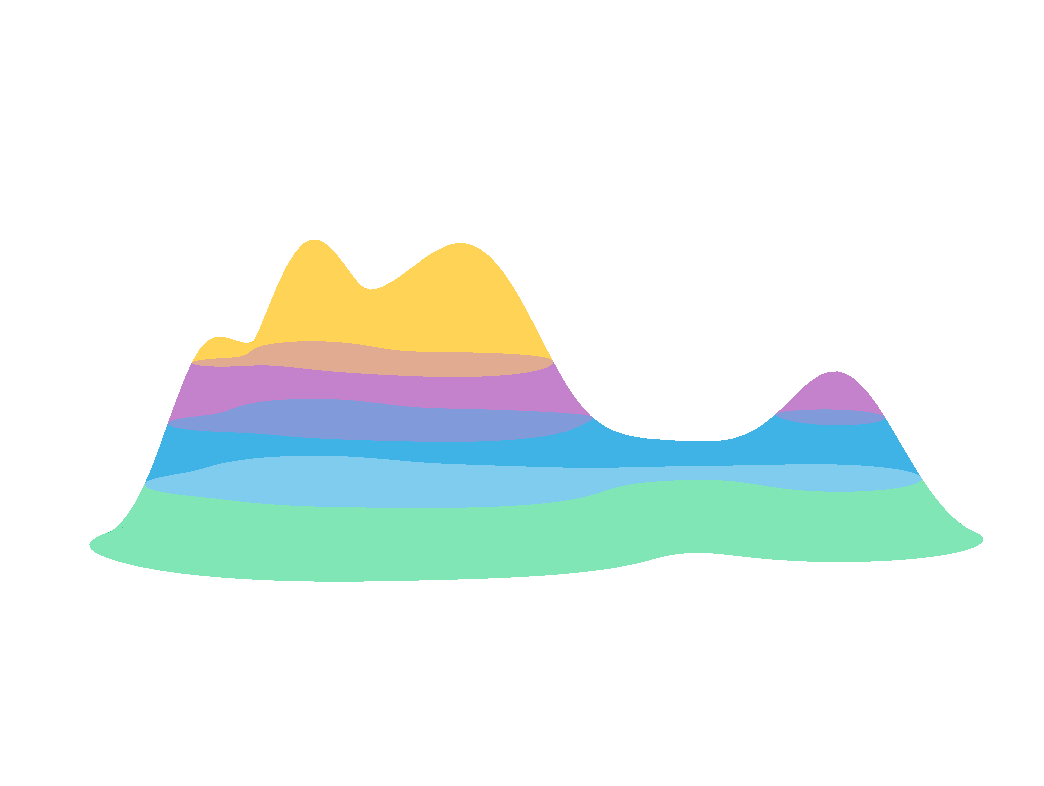
\includegraphics[trim=50 190 0 200, clip, scale=0.2]{scripts/figures/scalar.png}
    % 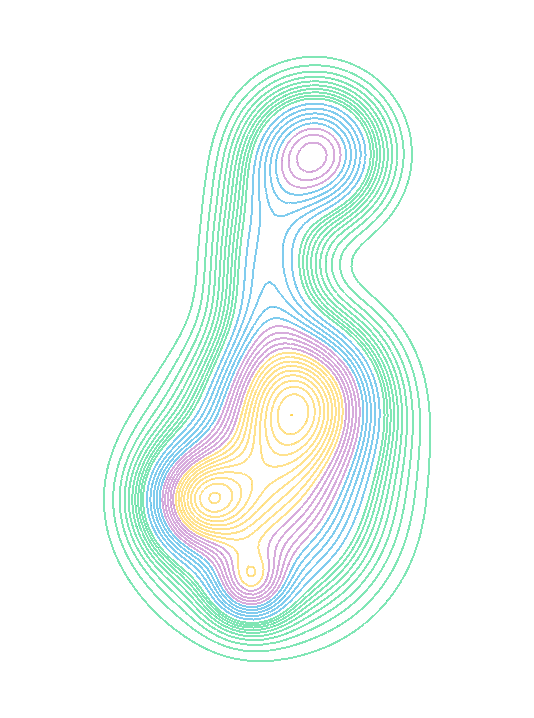
\includegraphics[trim=100 25 75 0, clip, angle=280, scale=0.25]{scripts/figures/scalar_contour.png}
    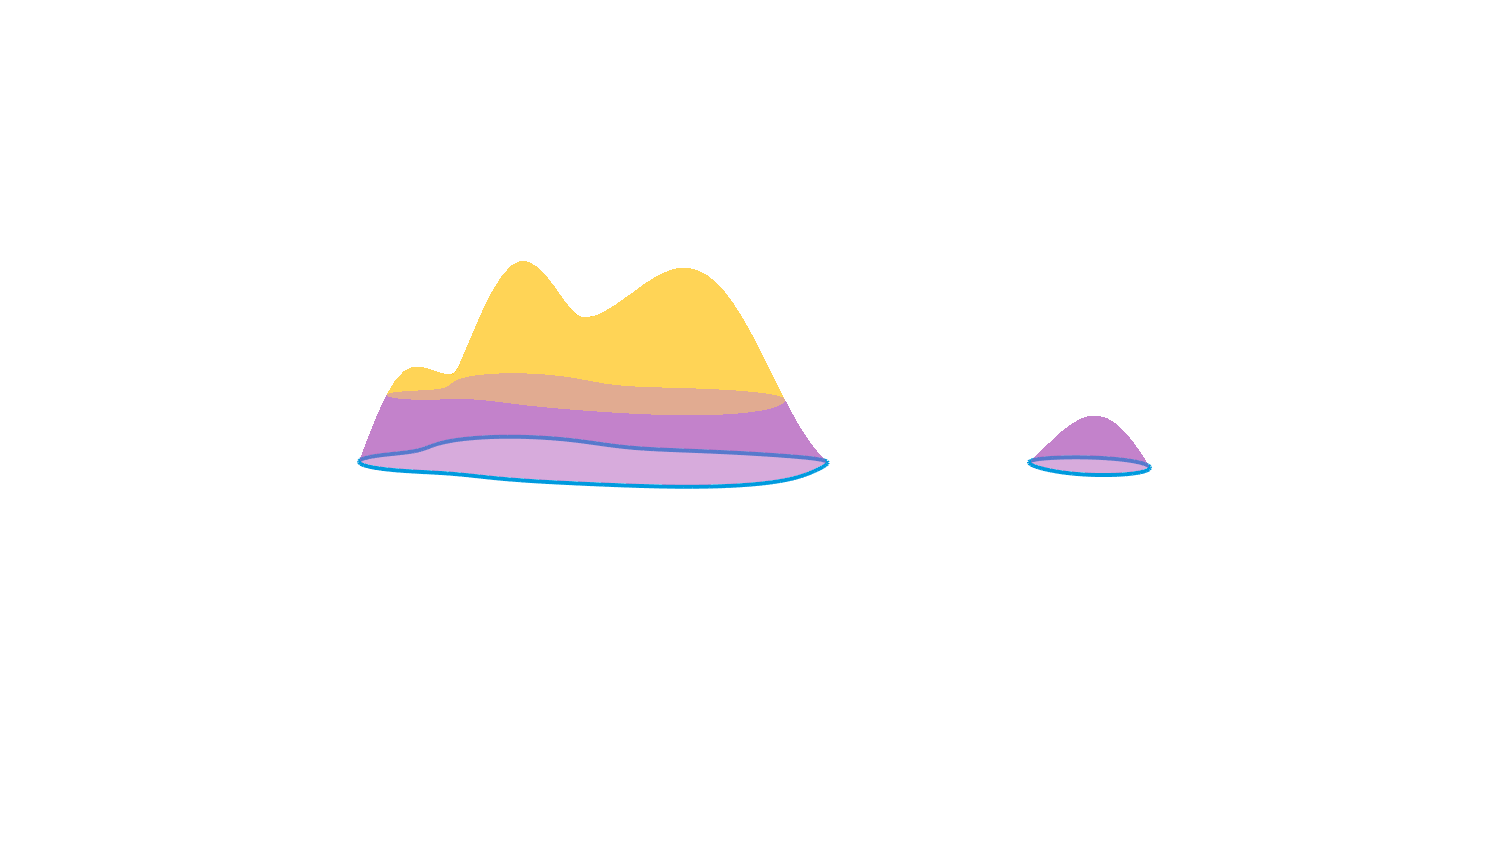
\includegraphics[trim=200 300 200 200, clip, width=0.5\textwidth]{../scripts/figures/surf/ass1_C_side.png}
    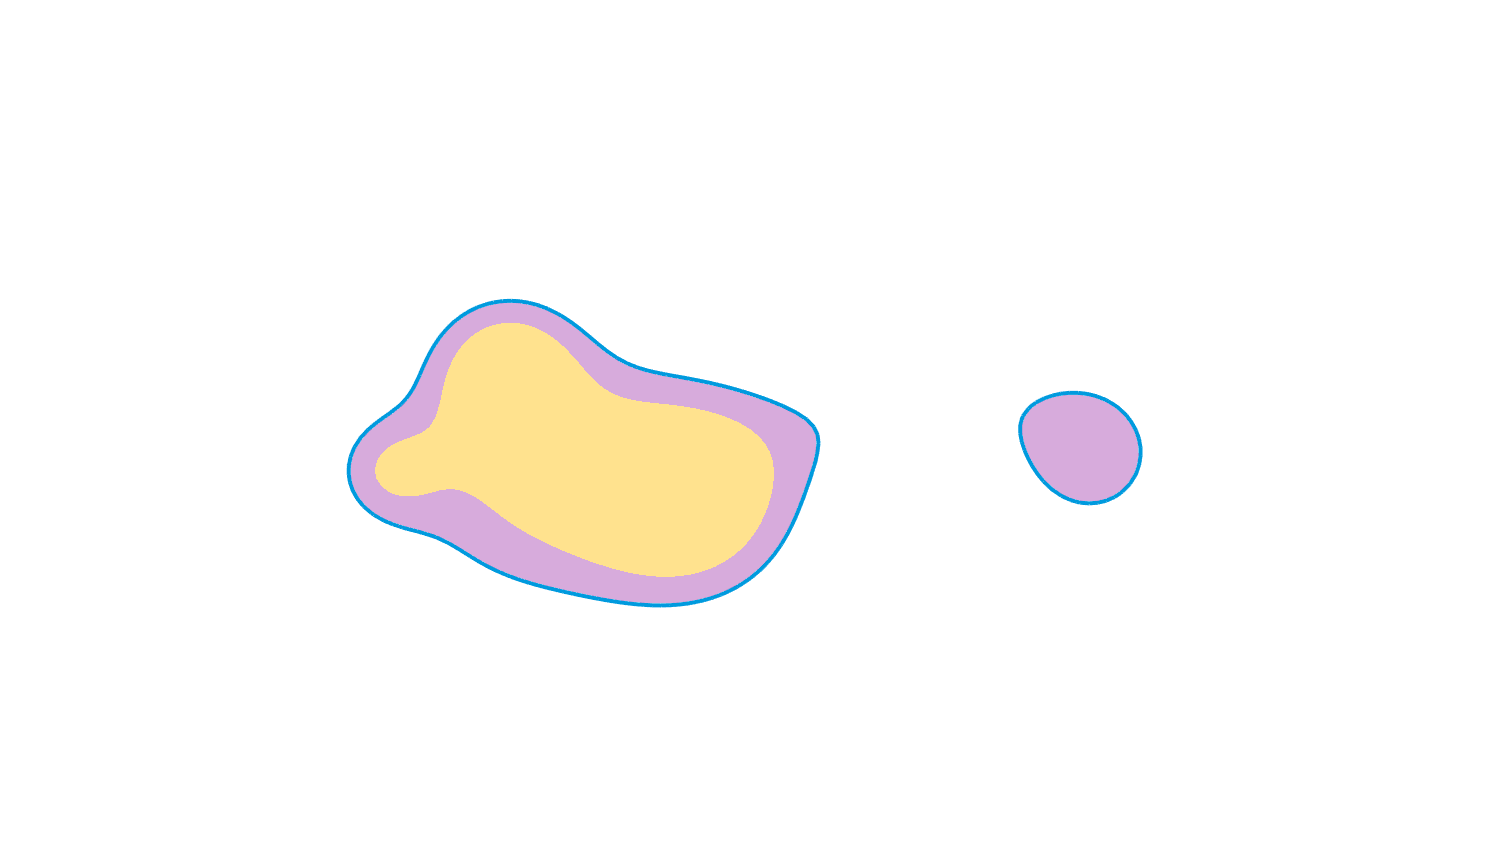
\includegraphics[trim=300 150 200 200, clip, width=0.3\textwidth]{../scripts/figures/surf/ass1_C_top.png}
    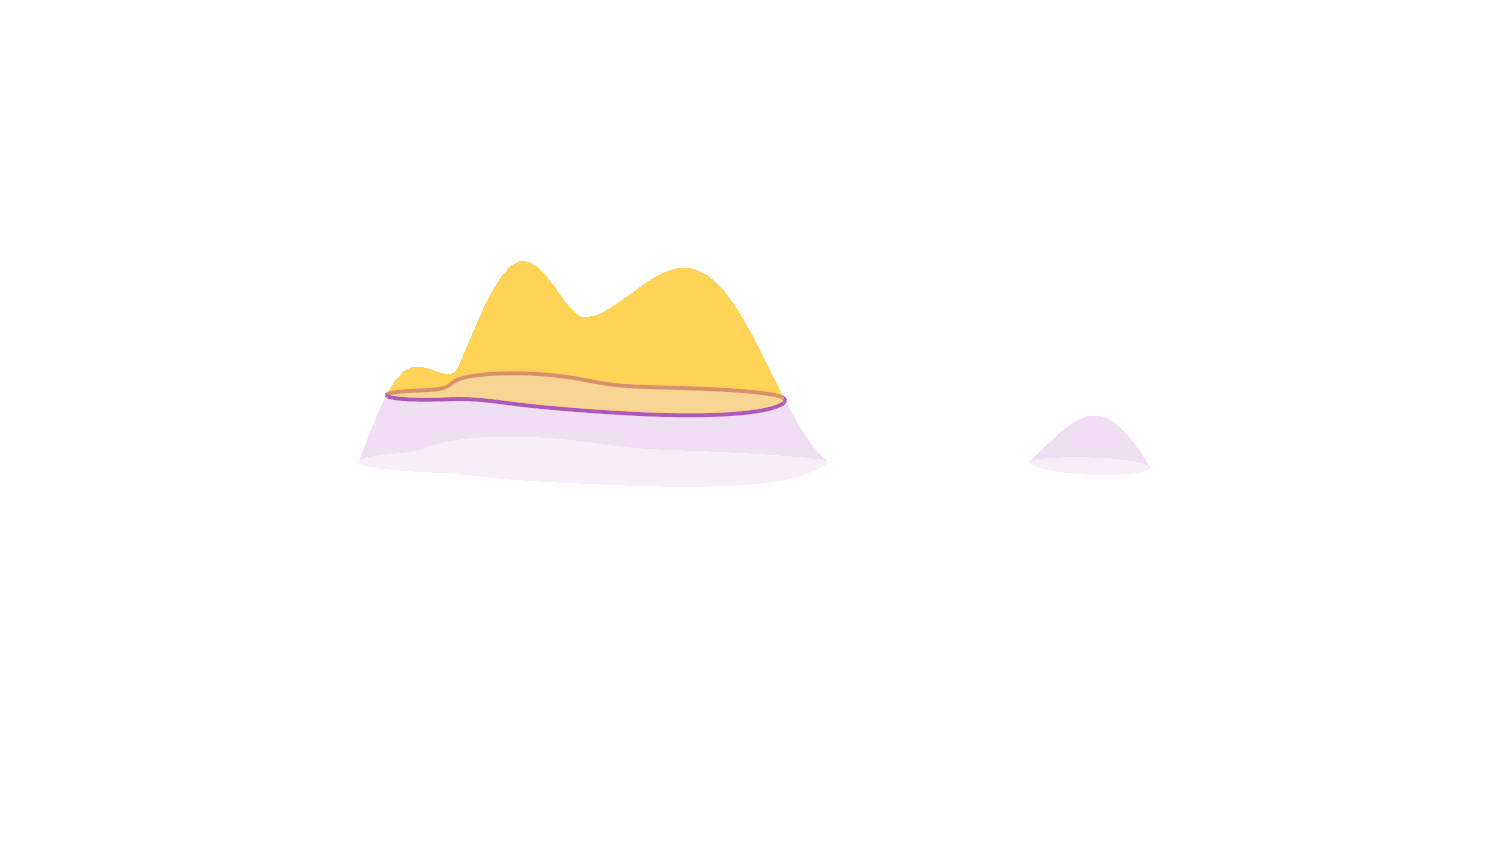
\includegraphics[trim=200 300 200 200, clip, width=0.5\textwidth]{../scripts/figures/surf/ass1_D_side.png}
    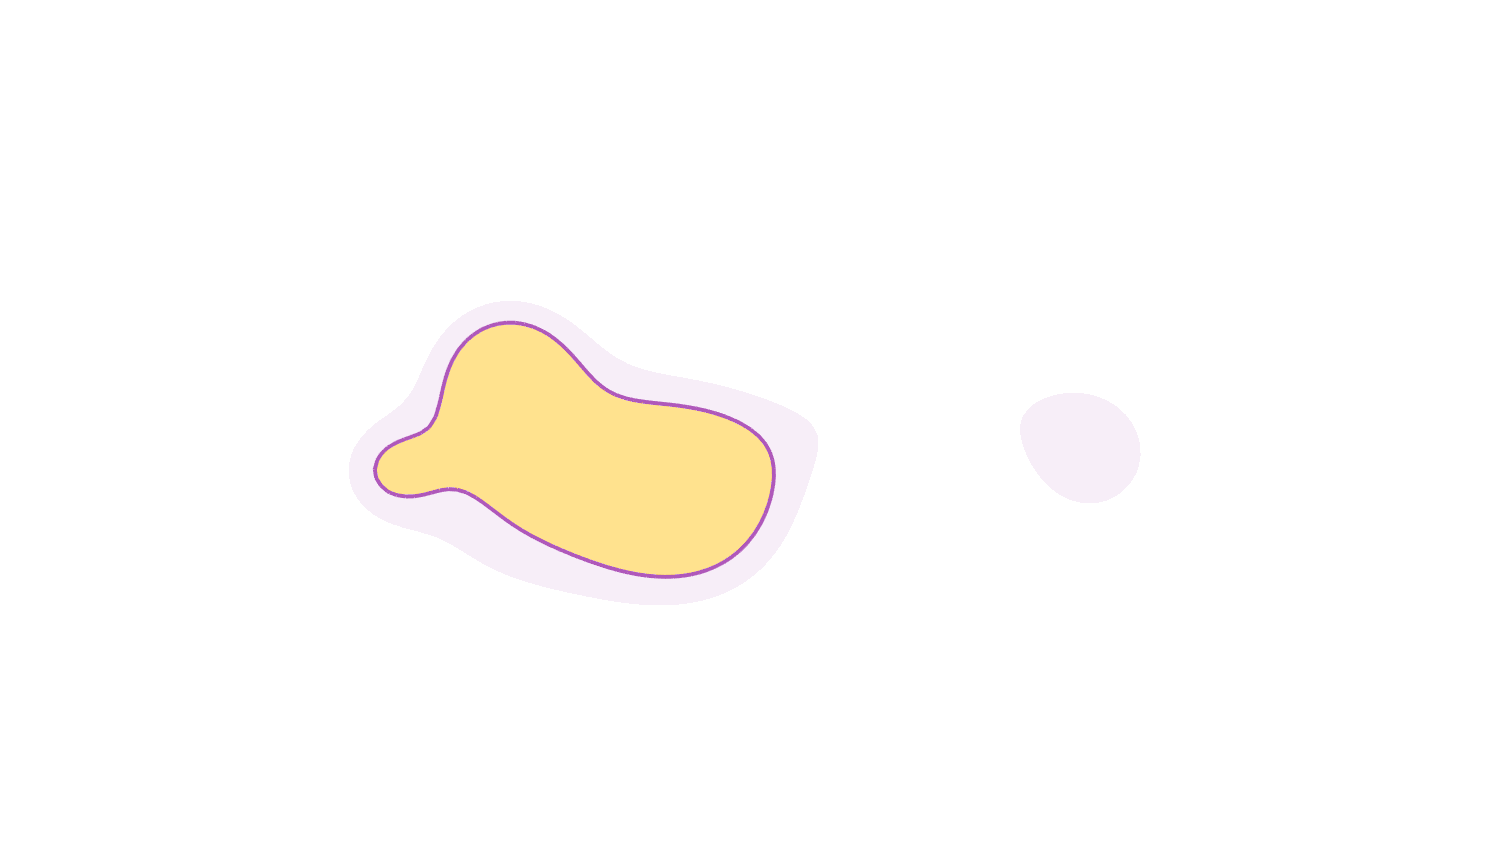
\includegraphics[trim=300 150 200 200, clip, width=0.3\textwidth]{../scripts/figures/surf/ass1_D_top.png}
    % 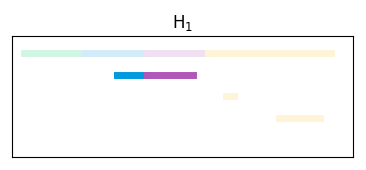
\includegraphics[scale=0.7]{scripts/figures/scalar_barcode_H1-masked.png}
  \end{textblock*}
\end{frame}

\begin{frame}
  \frametitle{{\small Assumption 1 and the Geometric TCC}}

  % \[\begin{tikzcd}
  %   \hom_0(\overline{B_{\omega+c(\delta+\zeta)}},\overline{D})\arrow{d}{m} \arrow{r}{j} &
  %   \hom_0(\overline{B_\omega}, \overline{D}) \arrow{d}{\ell} \\
  %   %
  %   \hom_0(\overline{Q_{\omega+c\delta}^\delta}, \overline{P^\delta}) \arrow{r}{i} &
  %   \hom_0(\overline{Q_{\omega-c\zeta}^\delta}, \overline{P^\delta}).
  % \end{tikzcd}\]

  \begin{theorem}[Geometric TCC]
    % Let $j : \hom_0(\cmp{B_{\omega+c(\delta+\zeta)}},\cmp{D})\to \hom_0(\cmp{\B},\cmp{D})$ and $i : \hom_0(\cmp{\QQ^\of}, \cmp{P^\of})\to \hom_0(\cmp{\Q^\of}, \cmp{P^\of})$ be induced by inclusion.
    %
    If $j$ is surjective and $\mathbf{rk}~i\geq \mathbf{rk}~j$ then $D\setminus B_\omega\subseteq P^\delta$ and $Q_{\omega-c\zeta}^\delta$ surrounds $P^\delta$ in $D$.
  \end{theorem}
\end{frame}

\begin{frame}
  \frametitle{{\small Duality, Assumption 2, and the Algorithmic TCC}}

  % \begin{itemize}
  %   \item Can't compute homology of complements: duality
  %   \item don't know number of connected components: assumption 2
  %   \item Rips-\v Cech interleaving and the Algorithmic TCC
  % \end{itemize}

  \textbf{Duality:} $\hom_d(P^\e,Q_z^\e)\cong\hom_0(D\setminus Q_z^\e, D\setminus P^\e)$.

  % \begin{textblock*}{12cm}(1cm,4.5cm)
  %
  % \end{textblock*}
\end{frame}


\begin{frame}
  \frametitle{{\small Duality, Assumption 2, and the Algorithmic TCC}}

  % \begin{itemize}
  %   \item Can't compute homology of complements: duality
  %   \item don't know number of connected components: assumption 2
  %   \item Rips-\v Cech interleaving and the Algorithmic TCC
  % \end{itemize}

  \only<1>{\begin{textblock*}{11cm}(1cm,2cm)
    \textbf{Assumption 2:} $\hom_0(D\setminus B_\omega\hookrightarrow D\setminus B_{\omega-c(\delta+\zeta)})$ is \emph{injective}.
  \end{textblock*}}

  \begin{textblock*}{12cm}(1cm,4.5cm)
    \includegraphics<1>[trim=200 300 200 200, clip, width=0.5\textwidth]{../scripts/figures/surf/ass2_C_side.png}
    \includegraphics<1>[trim=300 200 200 200, clip, width=0.3\textwidth]{../scripts/figures/surf/ass2_C_top.png}
    \includegraphics<1>[trim=200 300 200 200, clip, width=0.5\textwidth]{../scripts/figures/surf/ass2_B_side.png}
    \includegraphics<1>[trim=300 200 200 200, clip, width=0.3\textwidth]{../scripts/figures/surf/ass2_B_top.png}
  \end{textblock*}

  \only<2>{\begin{lemma}\label{lem:assumption2}
    If $\hom_0(D\setminus B_\omega\hookrightarrow D\setminus B_{\omega+c(\delta+\zeta)})$ is injective and each component of $D\setminus B_\omega$ contains a point in $P$ then $\mathbf{dim}~\hom_0(\rips^\delta(P\setminus Q_{\omega-c\zeta})) \geq \mathbf{dim}~\hom_0(D\setminus B_\omega)$.
  \end{lemma}}
\end{frame}

\begin{frame}
  \frametitle{{\small Duality, Assumption 2, and the Algorithmic TCC}}

  % \begin{itemize}
  %   \item Can't compute homology of complements: duality
  %   \item don't know number of connected components: assumption 2
  %   \item Rips-\v Cech interleaving and the Algorithmic TCC
  % \end{itemize}
  \begin{small}
    \[ \hom_k(\rips^\e(P, Q_w))\xrightarrow{J_w^\e}\hom_k(\cech^\e(P, Q_w))\xrightarrow{I_w^\e}\hom_k(\rips^\e(P, Q_w))\]
    % so
    % \[\mathbf{rk}~\hom_d(\cech^{\delta}(P, Q_{\omega-c\zeta})\hookrightarrow\cech^{\delta}(P, Q_{\omega+c\delta})) \geq\mathbf{rk}~ \hom_d(\rips^{\delta}(P, Q_{\omega-c\zeta})\hookrightarrow\rips^{2\delta}(P, Q_{\omega+c\delta}))\]

    \begin{theorem}[Algorithmic TCC]\label{thm:algo_tcc}
      Suppose $\hom_0(D\setminus B_{\omega+c(\delta+\zeta)}\hookrightarrow D\setminus B_\omega)$ is surjective and $\hom_0(D\setminus B_\omega\hookrightarrow D\setminus B_{\omega-c(\delta+\zeta)})$ is injective.

       If $\mathbf{rk}~\hom_d(\rips^\delta(P, Q_{\omega -c\zeta})\hookrightarrow \rips^{2\delta}(P, Q_{\omega+c\delta})) \geq \mathbf{dim}~\hom_0(\rips^\delta(P\setminus Q_{\omega-c\zeta}))$ then $D\setminus B_\omega\subseteq P^\delta$ and $Q_{\omega-c\zeta}^\delta$ surrounds $P^\delta$ in $D$.
    \end{theorem}
  \end{small}

  % \begin{textblock*}{12cm}(1cm,4.5cm)
  %
  % \end{textblock*}
\end{frame}

% !TeX root = ../main.tex

\begin{frame}
  \frametitle{Persistent Homology and Interleaving}

  \begin{itemize}
    \item The idea of Persistent Homology,
    \item Persistence modules and interleaving,
    \item Interleaving surrounding pairs,
    \item Proof sketch.
  \end{itemize}
\end{frame}


% \section{Section I : History}
%
% \subsection{SubSection A}
%
% \begin{frame}
%   \frametitle{Who?}
%   \begin{block}{A block}
%   Just a block
%   \end{block}
% \end{frame}
%
% \subsection{SubSection B}
% \begin{frame}
%   \frametitle{What?}
%   \begin{theorem}
%   Perhaps a theorem?
%   \end{theorem}
% \end{frame}
%
% \subsection{SubSection C}
% \begin{frame}
%   \frametitle{When?}
%   \begin{exampleblock}{Example 1}
%   Perhaps an example?
%   \end{exampleblock}
% \end{frame}
%
% \subsection{SubSection D}
% \begin{frame}
%   \frametitle{Where?}
%   \begin{block}{A small table}
%   \begin{center}
%   \begin{tabular}{ccc}
%   \toprule
%   Method & $x$ & $y$ \\
%   \midrule
%   Mine  & 1.23 & 4.56 \\
%   Yours & 2.34 & 5.68 \\
%   \bottomrule
%   \end{tabular}
%   \end{center}
%   \end{block}
% \end{frame}
%
% \section{Section II : Solution}
% \subsection{SubSection A}
%
% \begin{frame}
%   \frametitle{Who?}
% \end{frame}
%
% \subsection{SubSection B}
% \begin{frame}
%   \frametitle{What?}
% \end{frame}
%
% \subsection{SubSection C}
% \begin{frame}
%   \frametitle{When?}
% \end{frame}
%
% \subsection{SubSection D}
% \begin{frame}
%   \frametitle{Cost?}
% \end{frame}

\end{document}
